\documentclass[12pt]{article}

\usepackage{graphics}
\usepackage{epsfig}
\usepackage{times}
\usepackage{amsmath}
%\usepackage{float}  % for floating figures
\usepackage{floatrow} %for caption of figures on its side
\usepackage{natbib}  %for \citep
\usepackage{gensymb} %for \degree
\usepackage{subcaption} %for figures side by side

%%------------------------------------------------
%   For trackchanges package
%   Change the editor name as you like
%%------------------------------------------------
\usepackage[inline]{trackchanges}
\addeditor{XT}
\addeditor{EC}
%%------------------------------------------------
% Try one of these commands:
%     \add[editor]{added text}
%     \remove[editor]{removed text}
%     \change[editor]{removed text}{added text}
%     \note[editor]{note text}
%     \annote[editor]{text to annotate}{note text}
%%------------------------------------------------

% Borrowed the template from the CS dept. of Columbua University.
% <http://psl.cs.columbia.edu/phdczar/proposal.html>:
%
% The standard departmental thesis proposal format is the following:
%        30 pages
%        12 point type
%        1 inch margins all around = 6.5   inch column
%        (Total:  30 * 6.5   = 195 page-inches)
%
% For letter-size paper: 8.5 in x 11 in
% Latex Origin is 1''/1'', so measurements are relative to this.

\topmargin      0.0in
\headheight     0.0in
\headsep        0.0in
\oddsidemargin  0.0in
\evensidemargin 0.0in
\textheight     9.0in
\textwidth      6.5in

\title{{\bf 3D Numerical Models for Along-axis Variations in Diking at Mid-Ocean Ridges} \\
\it Thesis proposal}

\author{ {\bf Xiaochuan Tian}  \\
Center for Earthquake Research and Information \\
The University of Memphis\\
{\small xtian@memphis.edu}
}
\date{\today}

\begin{document}
\pagestyle{plain}
\pagenumbering{roman}
\maketitle

\pagebreak
\begin{abstract}

Bathymetry of ocean floors reveals a great variety of morphologies at Mid-ocean Ridges (MORs). Previous studies showed that the morphologies at slow spreading MORs are mainly controlled by the ratio between rates of magma supply and plate extension. 2D models for the across-ridge cross-sections have been successful in explaining many of the observed morphological features such as abyssal hills and oceanic core complexes. However, the magma supply varies along the ridge and the interaction between the tectonic plates and magmatism at MORs are inevitably 3D processes. We propose to investigate the consequences of the along-axis variability in diking in terms of faulting pattern and the associated structures. This work will include implementation of an algorithm of parameterizing repeated diking in a 3D parallel geodynamic modeling code.

\end{abstract}

\pagebreak
\tableofcontents
\pagebreak

\cleardoublepage
\pagenumbering{arabic}

\section{Introduction}
\label{ch:intro}

Around 70\% of the Earth's crust is oceanic crust and the mid-ocean ridges (MORs), the longest mountain chains on the Earth, are where new crust are forming with a multitude of seismic and volcanic activities. To study how new crust is created and how MORs evolve is significant for Earth Sciences.  Geodynamic modeling along with a variety of geological, geophysical observation and lab experiment constraints have been used to study how the MORs work as a system under geological time scale.

High-resolution multi-beam bathymetry has revealed various characteristics of topography along and across MOR axis. Three specific questions stimulate people's interests most. First, what causes the distinct difference in axial topography between slow and fast spreading ridges. Second, for slow spreading ridges, why does topography along ridge varies and how to explain many features observed. Third, why do oceanic core complexes (OCCs) form and what is the mechanism. 

%\subsection{Background}
%\label{ch:back}
According to \citep{Fowler2004}, variations in  mid-ocean ridge morphologies are mainly controlled by four factors: magma supply, tectonic strain, hydrothermal circulation and spreading rate. Among them, the spreading rate is the most important. Slow-to-intermediate spreading centers (half spreading rate less than 4cm/year) produce median valleys that are typically 10$\sim$20km wide and 1$\sim$2km deep (e.g., Mid-Atlantic Ridges, Figure 1(a)). Fast-spreading centers (half spreading rate greater than 5cm/year) have axial highs that are 10$\sim$20 km wide, 0.3$\sim$0.5 km high (e.g., East Pacific Rise, Figure 1(b)).

\begin{figure}[H]
\centering
\begin{subfigure}{.5\textwidth}
  \centering
  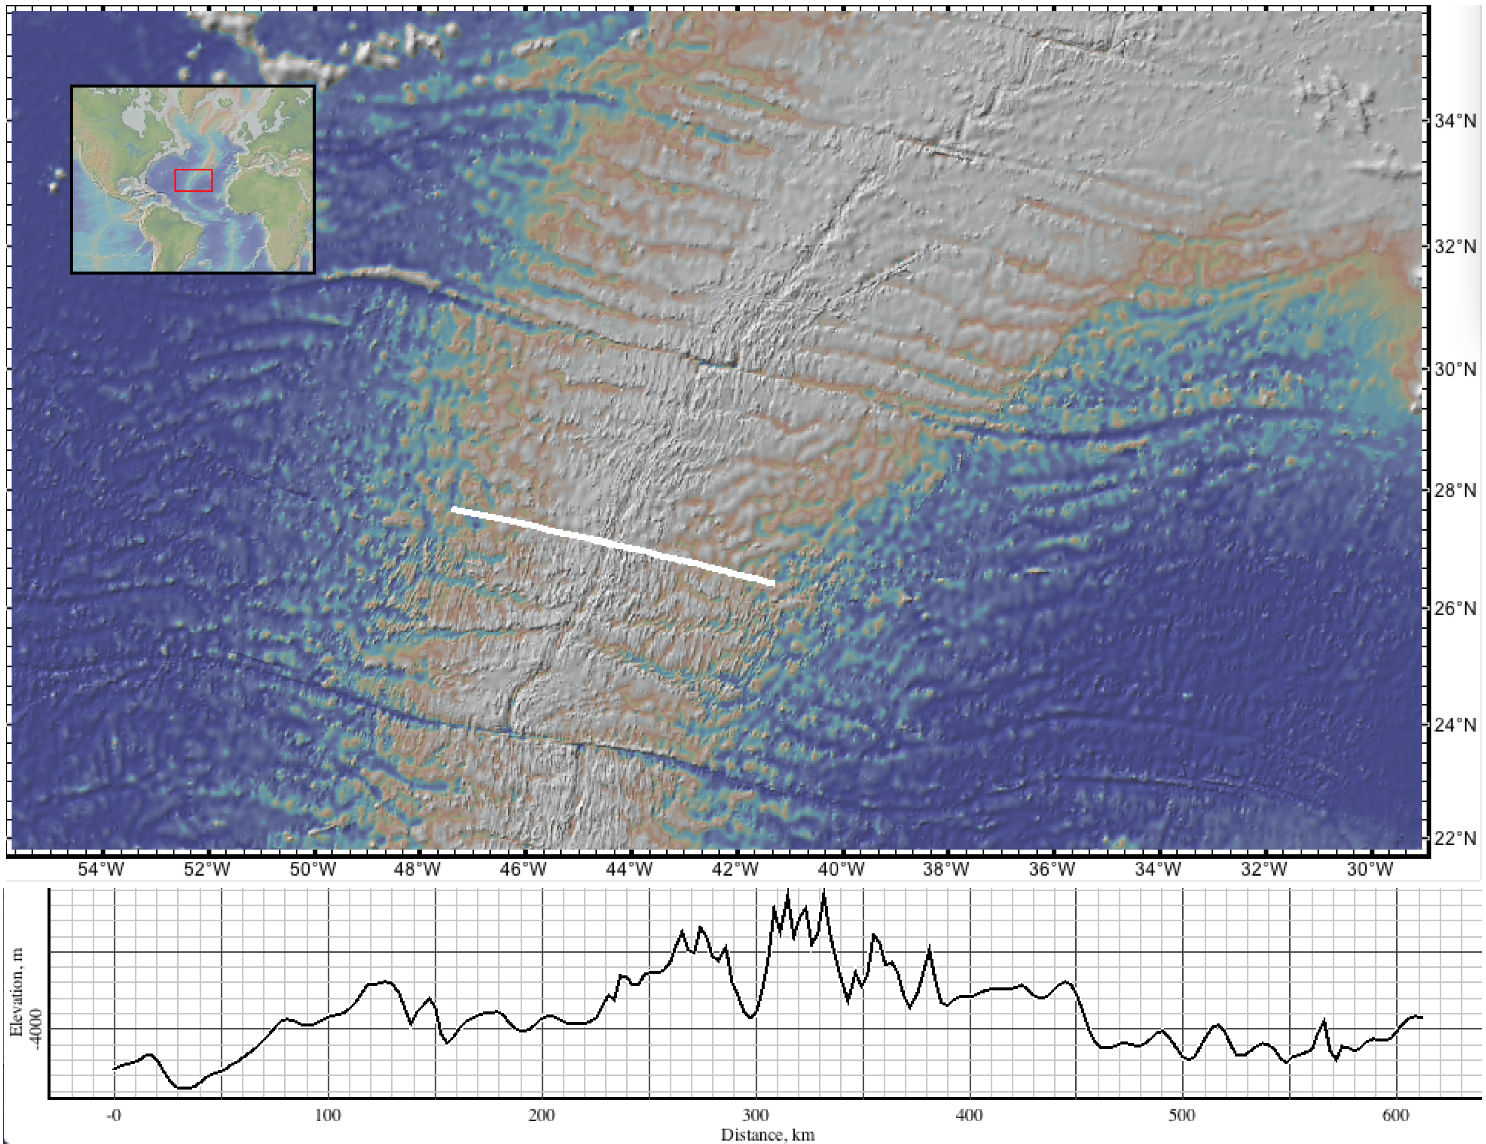
\includegraphics[width=.8\linewidth]{fig1_1.png}
  \caption{\small{Slow spreading Mid-Atlantic Ridge}}
  \label{fig1_1}
\end{subfigure}%
\begin{subfigure}{.5\textwidth}
  \centering
  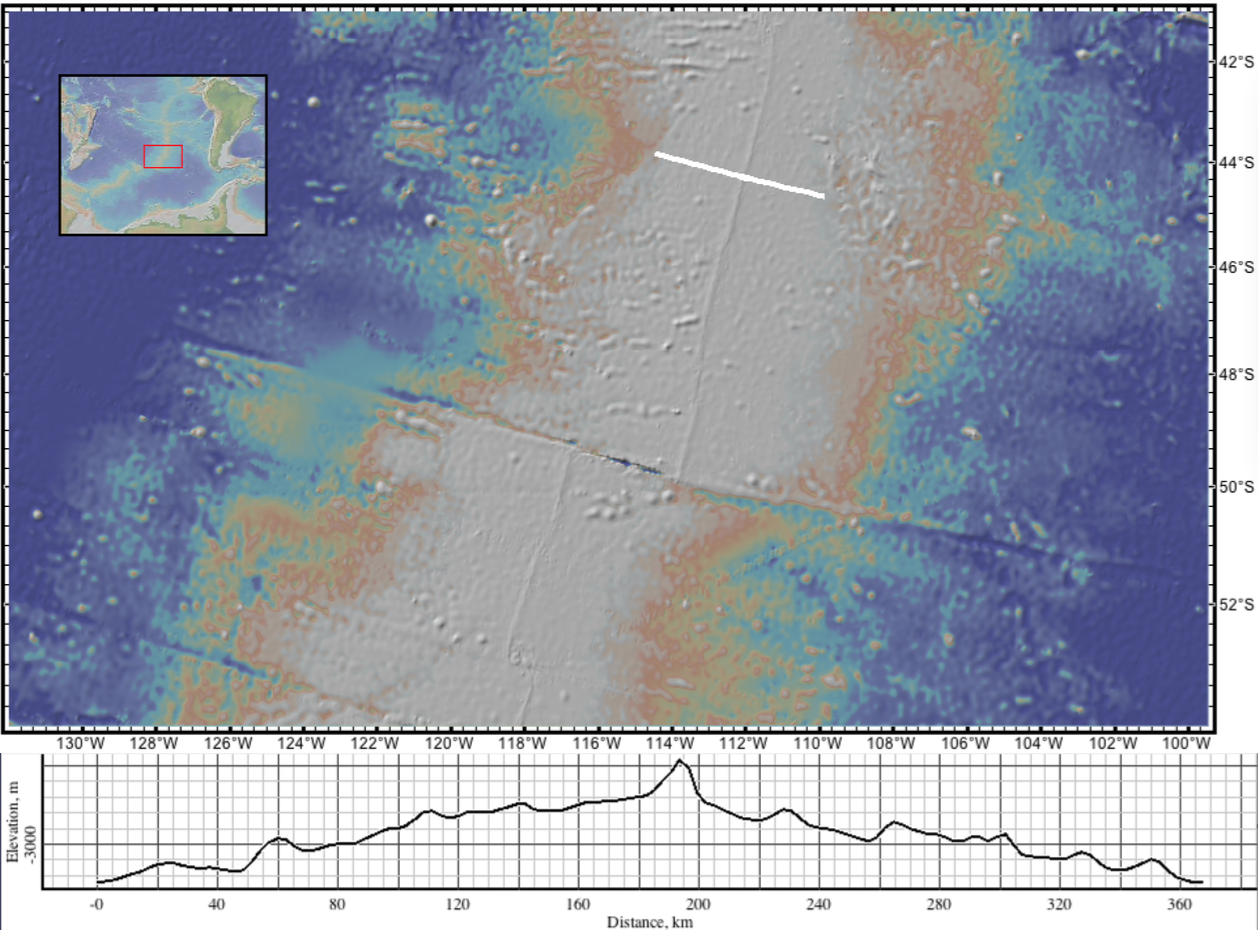
\includegraphics[width=.8\linewidth]{fig1_3.png}
  \caption{\small{Fast spreading East Pacific Rise}}
  \label{fig1_3}
\end{subfigure}
\caption{\small{Profiles of bathymetry across MORs.}}
\label{fig1}
\end{figure}
Slow spreading ridges exhibit along-axis variations as well in terms of the width and depth of median valleys and the off-axis morphology.  Figure~\ref{fig2_1} shows that the topographic profile nearer to the center of the ridge segment (A-A') is rather symmetric and has higher frequency. The maximum relief is about 1km. In constrast, the near-tip profile (B-B') is asymmetric and has much lower frequency and a greater relief ($\sim$3km). The bathymetry and crustal thickness along the ridge valley also varies. From \citep{Chen1999}, the maximum along-axis variation in crustal thickness $\Delta H_{c}$ is linearly increasing with segment length $L$, and the relationship is $\Delta H_{c}(L)=0.0206L$ (Figure~\ref{fig3_1}).

\begin{figure}[H]
 \centering
  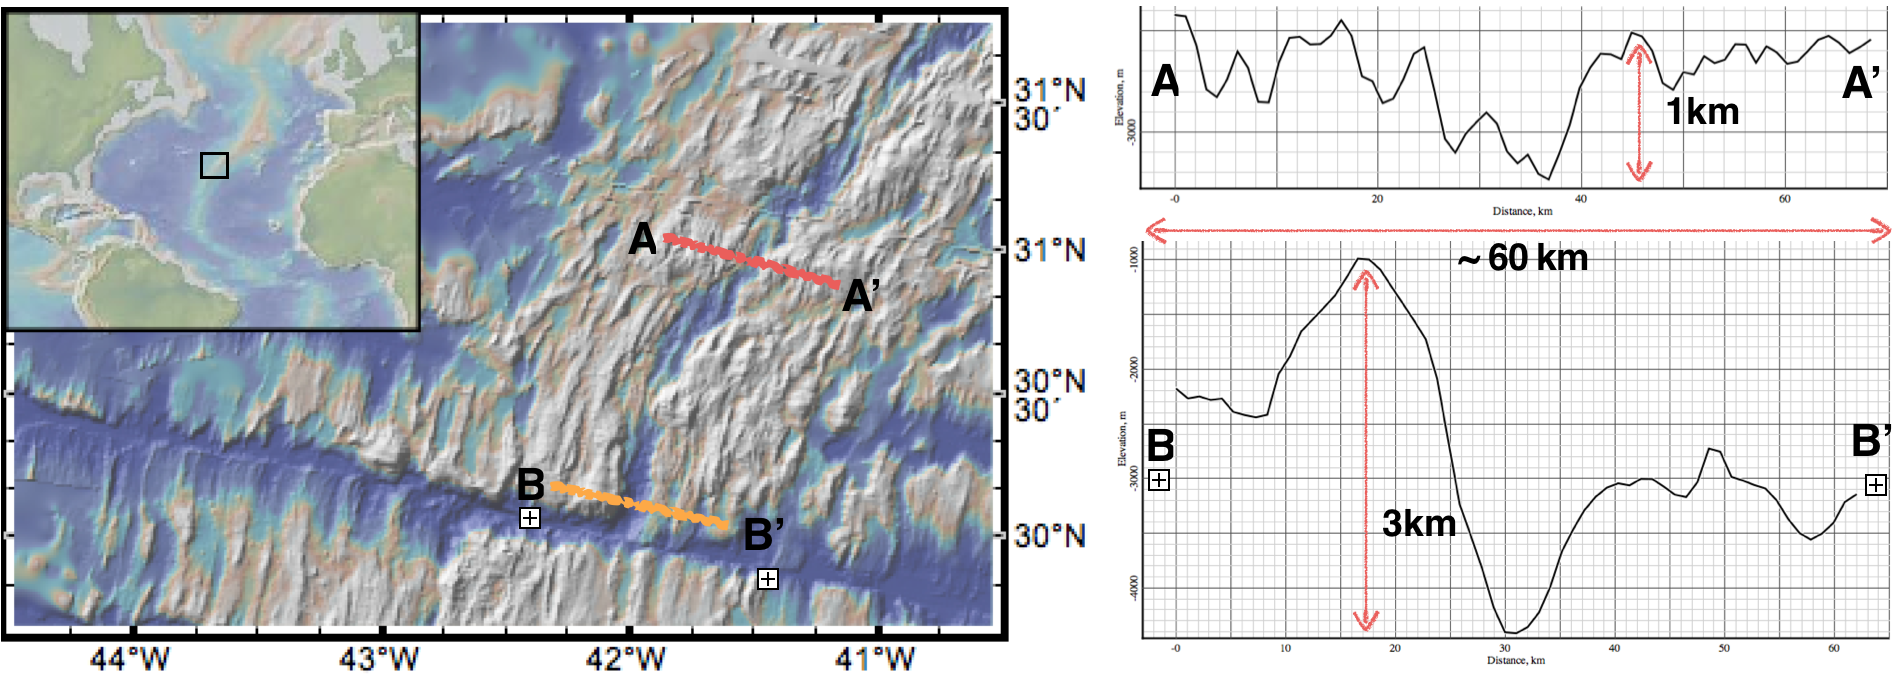
\includegraphics[scale=0.4]{fig2_1.png}
 \caption{\small{Two bathymetry cross-sections of Mid-Atlantic Ridge (MAR) with 10 times vertical exaggeration. A-A' is closer to the ridge segment center while B-B' is at the tip of the segment near the Atlantis Transform fault.}}
 \label{fig2_1}
\end{figure}

\begin{figure}[H]
 \centering
  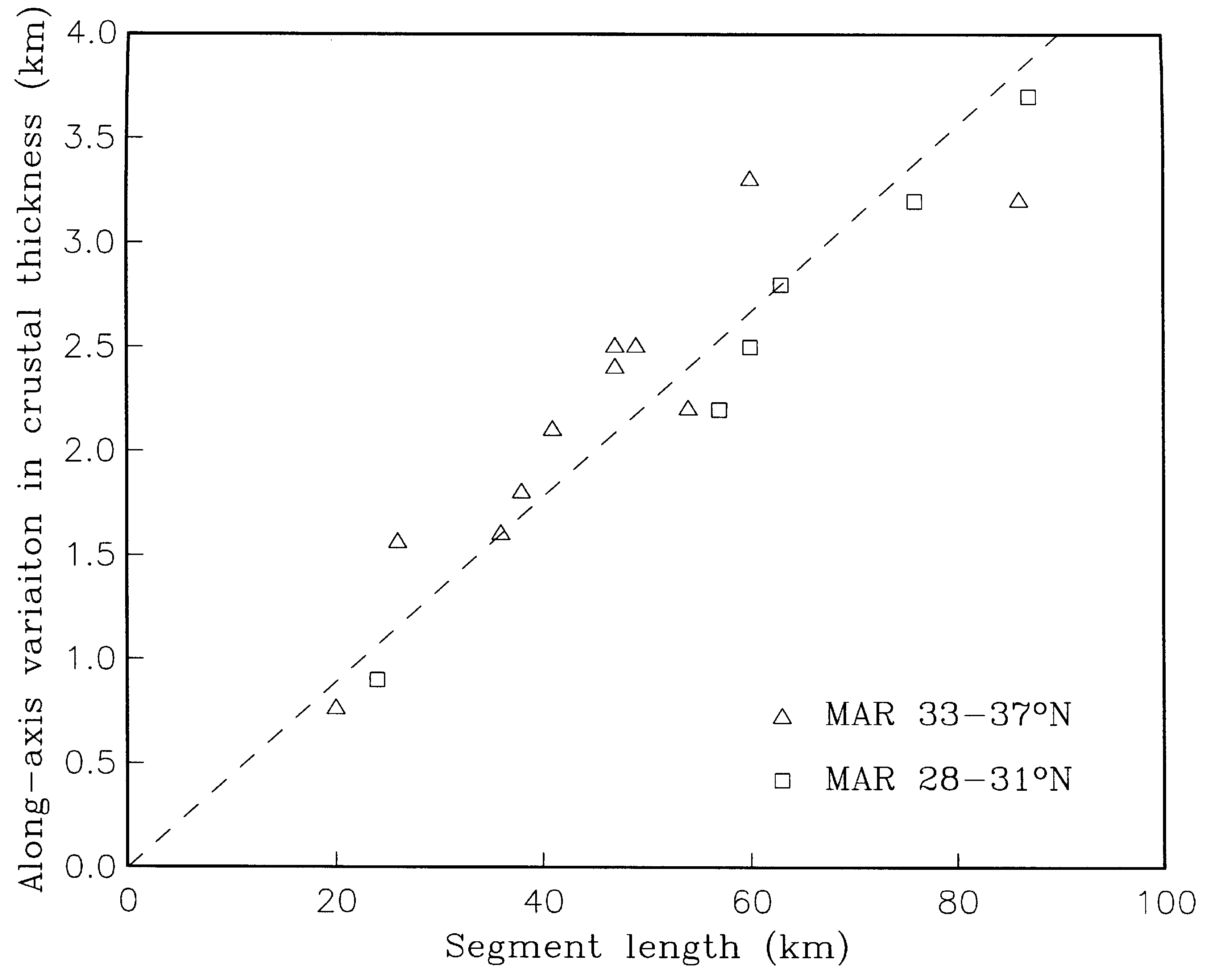
\includegraphics[scale=0.3]{fig3_1.png}
 \caption{\small{Relationship between the maximum crustal thickness variations along a ridge segment and the segment length.The dashed line is the best-fit linear regression of the combined data. \citep{Chen1999}}}
 \label{fig3_1}
\end{figure}

%Moreover, a 3D view of B-B' area of Figure~\ref{fig2_1} shows the 20km wide, 25km long and 3km relief Atlantis Massif. The huge geologic structure is a window for learning lower crust and upper mantle because it is believed to be a result of exhumation of deeper material to the seafloor through tectonic processes.
%
%\begin{figure}[H]
% \centering
%  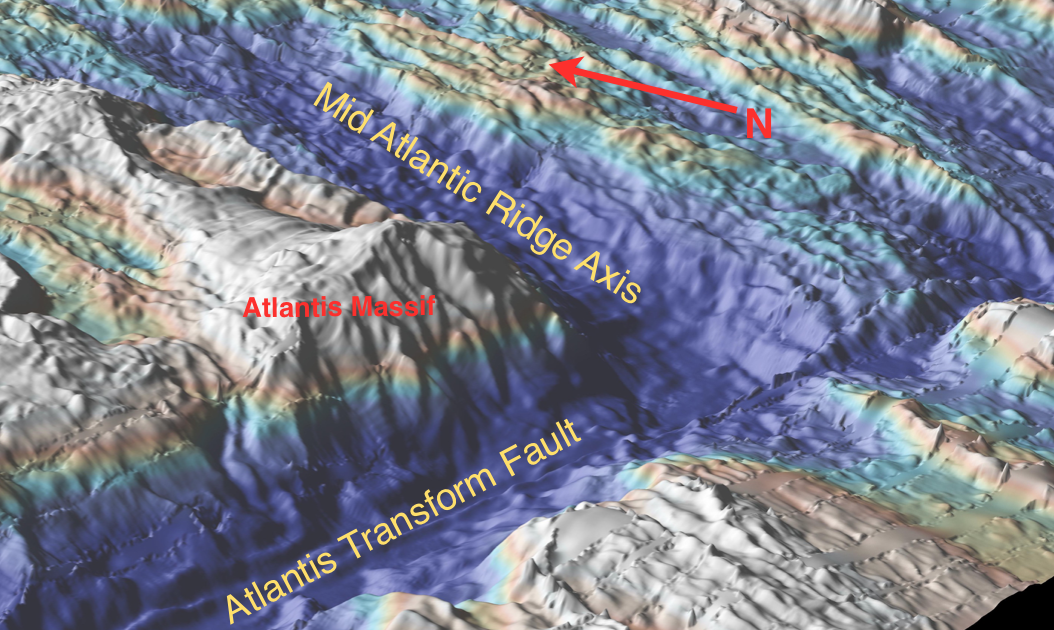
\includegraphics[scale=0.4]{fig4_1.png}
% \caption{\small{Zoom in B-B' area, a 3D view of Atlantis Massif.}}
% \label{fig4_1}
%\end{figure}

%\subsection{Related work}
%\label{ch:related}
Magma supply at MORs is mostly a passive process when no hot plume presents \citep{Fowler2004}. Hot mantle rises up to fill the vacated room being created by plate separation and decompression will lead to partial melting of the hot mantle. The melt upwells due to both pressure difference and buoyancy from lateral density difference. When the melt solidifies near the surface, it forms new crust. This diking process can also release extensional stresses result from far-field driving forces.

The passive nature of magma supply results in the major difference between fast and slow spreading ridges in the amount of magma supply. At the fast spreading ridges, magma supply is always sufficient for accommodating plate separation by filling the space by dikes. However, the amount of magma supplied in the form of dikes is not as much at slow spreading ridges and the oceanic lithosphere experiences internal deformations (i.e. tectonics process like normal faulting) when the accumulated extensional stress exceeds the strength of the crust. 

\citet{Buck2005} attributed the contrasting faulting patterns and ocean floor morphology of fast- and slow-spreading ridges to the difference in the amount of plate extension accommodated by diking. They defined the ratio between the rates of diking and plate separation as \change[XT]{M$=\Delta\varepsilon_{xx}/2V_{x}$}{M$=\Delta\dot{\varepsilon_{xx}}/2V_{x}$}, where \change[XT]{$\Delta\varepsilon_{xx}$}{$\Delta\dot{\varepsilon_{xx}}$} is the extensional strain \add[XT]{rate} due to the widening of diking \remove[XT]{ in a unit time }and $V_{x}$ is the half spreading rate of the MOR. According to this definition, M $=1$ represents the case where diking is frequent enough to release all the tensional stresses from plate separation. M $=0$ corresponds to the case of no magma supply, in which diking does not account for any of the plate motion and therefore plates kinematics requires plates to go through internal deformations. As shown in Figure~\ref{fig5_1}, an axial high forms at a fast spreading ridge \add[XT]{(M=1)} due to buoyancy from lateral density difference across ridge axis but a median valley forms at a slow-spreading ridge \add[XT]{(M=0.5)} due to near-axis normal faulting, which is in turn caused by the stretching of oceanic lithosphere.

%\citet[Buck2005}
%\annote[XT]{They didn't explicitly mention the ratio M, and they cannot remesh (the dike is not repeatedly widening), the dike in Poliakov and Buck is a vertical place where initial shear stress is set to zero and normal stress is set to be the same as lithostatic pressure, I guess it is still different with the following M we are going to describe, maybe Buck, 2005 is the first work to explicitly proposed M} {\note[EC]{I think M factor was originally proposed by Poliakov and Buck, 1998} }also showed that the ratio of the diking-accommodated portion to the total plate motion can efficiently parameterize the kinematics of repeated diking.}

\begin{figure}[H]
 \centering
  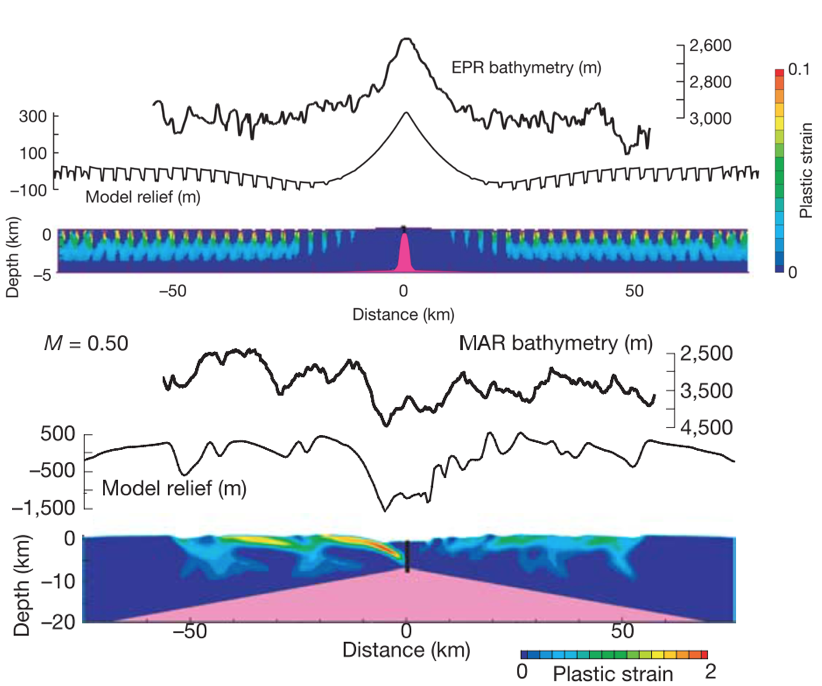
\includegraphics[scale=0.7]{fig5_1.png}
 \caption{\small{Upper one: modeling result for fast spreading agrees well with the observation of East Pacific Rise. Lower one: modeling result for slow spreading ridges agrees well with the bathymetry of Mid Atlantic Ridge. \citep{Buck2005}}}
 \label{fig5_1}
\end{figure}
\citet{Tucholke2008} expanded investigation on the role of M in the mid-ocean ridge mechanics. They focused on faulting behaviors of slow spreading ridges and find that the Oceanic Core Complexes (OCCs) are most likely to form when M varies from 0.3 to 0.5. As shown in Figure 5, when M=0.7, repeated diking pushes faults forming at the spreading center away from axis. Since the thickness of the brittle layer increases away from the ridge axis, frictional and bending energy for maintaining the fault also increases. When it exceeds the energy for breaking a new near-axis fault, the old fault will be replaced by the new one. When M=0.3$\sim$0.5, the normal faults remains active for a long time to become detachment faults, exhuming the lower crust and mantle materials to the seafloor. When M is less than 0.3, most of the tension is accommodated by intra-plate deformations rather than by diking and as a result, faulting pattern is more complicated and unsteady.

The M-factor formulation used in these previous 2D models successfully explained major features found in across-ridge profiles of seafloor bathymetry. However, 2D models have limitations in studying the along ridge-axis interactions, especially when important variables are not constant along the ridge axis. Magma supply at fast spreading ridges seems always sufficient for accommodating plate motions with little variation along the ridge axis. The relatively uniform topography along fast spreading ridges is considered to be consistent with the uniformly abundance of magma supply. However, along slow spreading ridges, bathymetry, gravity anomaly, reflection and refraction seismology show good correlation with variation in crustal thickness \citep{Ryan2009}, \citep{Chen1999}, \citep{Lin1990} and \citep{Tolstoy1993}. Because oceanic crust is mainly formed by upwelled magma at the ridge, variation in the thickness of the crust implies variation in magma supply. At slow spreading ridges, hydrothermal cooling, thermal structures and even local spreading rate [Baines2008] also varies both along and across the ridge axis and they appear interrelated. Thus, for slow-to-intermediate spreading ridges, the interactions between tectonics and magmatism at MORs are inevitably 3D processes and 3D numerical models are desirable for better understanding factors controlling both across- and along-ridge variations. 
\begin{figure}[H]
\floatbox[{\capbeside\thisfloatsetup{capbesideposition={right,bottom},capbesidewidth=5cm}}]{figure}[\FBwidth]
{\caption{\small A$\sim$F: Faulting behavior for different values of M. Geologic interpretation is superimposed on modeled distribution of strain rate. Dots show breakaways of initial faults. Dashed seafloor is original model seafloor, red dotted seafloor is formed dominantly by magmatic accretion, and solid bold is fault surface. Note that detachment faults in B and C are not interrupted by secondary faults. \citep{Tucholke2008}}}
 {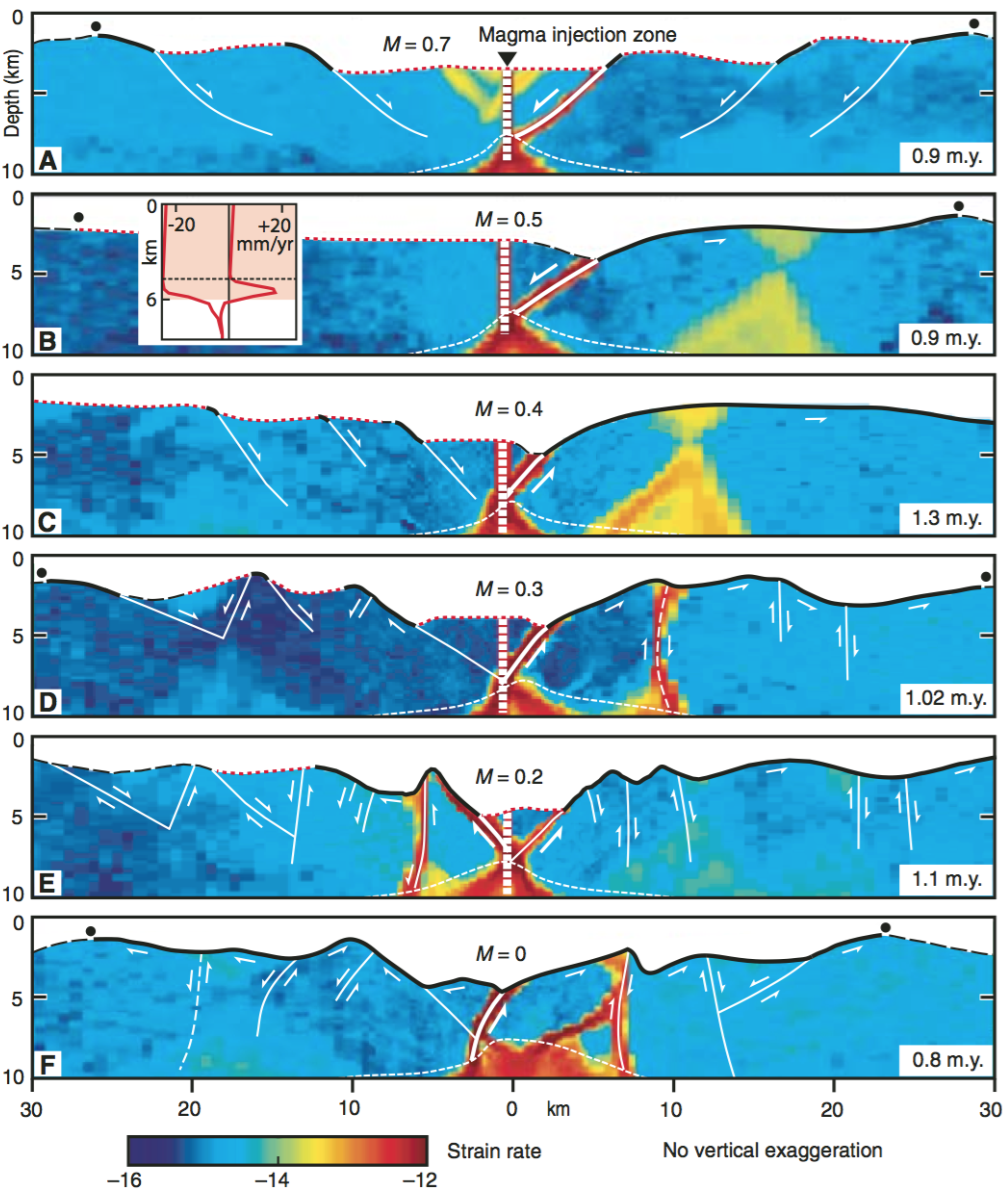
\includegraphics[width=10cm]{fig6_1.png}} 
 \label{fig6_1}
\end{figure}


\break
\section{Proposed Work}
\label{ch:purpose}

The purpose of this thesis is to study how the along-ridge variation in M will make a contribution to the observed various topography assuming that M is the first order control over the topography evolution of MORs governing the interaction between magmatism and tectonic deformations.
We will extend the M-factor formulation originally developed for 2D models to 3D by implementing it into a 3D numerical modeling code SNAC \citep{Choi2008}. We will focus on studying the last two questions mentioned in the introduction: 1) why does topography along ridge varies and how to explain many features observed; 2) why do OCCs form and what is the mechanism. 

By systematically exploring the behaviors of the 3D models and comparing them with observations, we will be able to better understand  how the mid-ocean ridge magmatism and tectonic deformations interact. 

\break
\subsection{Method of Approach}
\label{ch:method}

% I commented out because this is like a basic premise of any kind of modeling.
% Probably needless to say... --EC.
%
%The idea is that we \change[EC]{utilize}{start with constraining the initial and boundary conditions as well as model parameters with} geophysical observations and published results\remove[EC]{ to constrain the setups of the 3D model}. \change[EC]{By i}{I}teratively minimizing the gap between results from models and observations\change[EC]{, hopefully, a model with consistent results will be generated}{will bring our models close to that of the natural MORs}. Then, we will interpret the observations based on that model.

The numerical modeling code, SNAC, is an explicit Lagrangian finite element code. It solves the force balance equation for elasto-visco-plastic materials. Figure~\ref{fig7_1} shows major parts of the SNAC's algorithm. 

The boundary conditions of the model are shown in Figure~\ref{fig8_1}, the 60$\times$20$\times$20 km simulated oceanic crust and upper mantle is stretched with a half spreading velocity $V_{x}$ prescribed on both side walls; Winkler foundation is applied at the bottom of the model and simulated sea water hydrostatic pressure is added on the surface in terms of an opposite Winkler foundation; All six walls are shear-stress free. For each time step dt, strain and strain rates are updated. A constitutive model returns updated stresses corresponding to these deformation measures. Internal forces are then calculated from the update stresses, which is plugged into the momentum balance equation together with the body force term. Then, the net force divided by internal mass yields acceleration at a node point, which is time-integrated to velocity and displacement. 

A 3D domain is discretized into hexahedral elements, each of which is in turn divided into two sets of tetrahedra. This redundant discretization prevents faulting from favoring a specific direction or ``mesh grains''. 

Rheology for the oceanic lithosphere is assumed to be elasto-visco-plasticic. When viscosity is high at low temperature, the rheology essentially becomes the Mohr-Coulomb plasticity with strain softening and thus can create shear bands that behave like faults. When temperature is high and viscosity is low, the rheology becomes the Maxwell viscoelasticity and can model creeping flow. By assuming an appropriate initial temperature distribution, we can effectively set up a structure of a brittle lithosphere and a ductile asthenosphere. Rheological parameters are taken from previous studies that used a similar rheology [Buck 2005; Tuckholke et al., 2008] or from lab experiments \citep[e.g.,][]{Kirby1987}. 

For 3D diking processs, the expanding strain \add[XT]{rate} $\Delta\dot{\varepsilon_{xx}}$ results from M will lead to extra-stresses in all three directions $\Delta\sigma_{xx}$, $\Delta\sigma_{yy}$ and $\Delta\sigma_{zz}$ based on the constitutive equations $\sigma_{ij}=\delta_{ij}\lambda\varepsilon_{ij}+2\mu\varepsilon_{ij}$.

\begin{figure}[H]
 \centering
  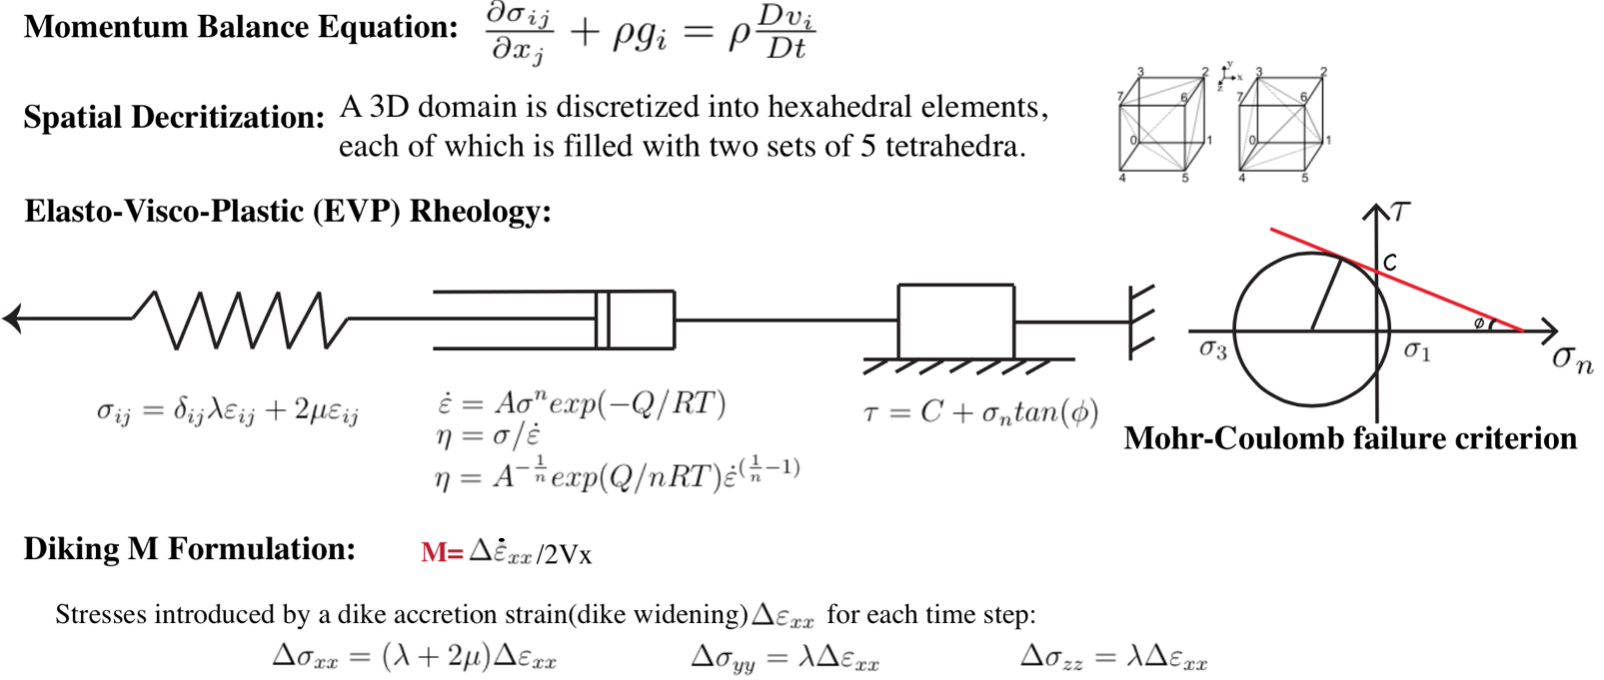
\includegraphics[scale=0.65]{fig7_2.png}
 \caption{\small{Essential components of the numerical method to be used for the proposed research}}
 \label{fig7_1}
\end{figure}

\subsection{Model Setup}

I propose the model setup shown in Figure~\ref{fig8_1}. Temperature linearly increases from 0 \degree C at the top surface to 240 \degree C at 6 km, reflecting enhanced cooling due to hydrothermal circulation. Below 6 km, the temperature profile follows the semi-infinite half-space cooling model of moving plates \citep[e.g.,][]{Turcotte2002}. For boundary conditions, free slip on two sides perpendicular to the $z$ coordinate axis. The top surface is traction-free and the bottom surface is supported by the Winkler foundation. Temperature is fixed at 0\degree C on the top surface and at 1300\degree C on the bottom surface. We will adopt the power-law rheology of \annote[EC]{dry diabase}{What did Buck et al. 2005 use? Usually, this is for oceanic crust but we don't have crust here...}\note[XT]{Buck et al., 2005 use dry diabase from kirby 1987, while Tucholke 2008 use dry diabase from Mackwell et al., 1998} \citep{Kirby1987}. 

\begin{figure}[H]
 \centering
  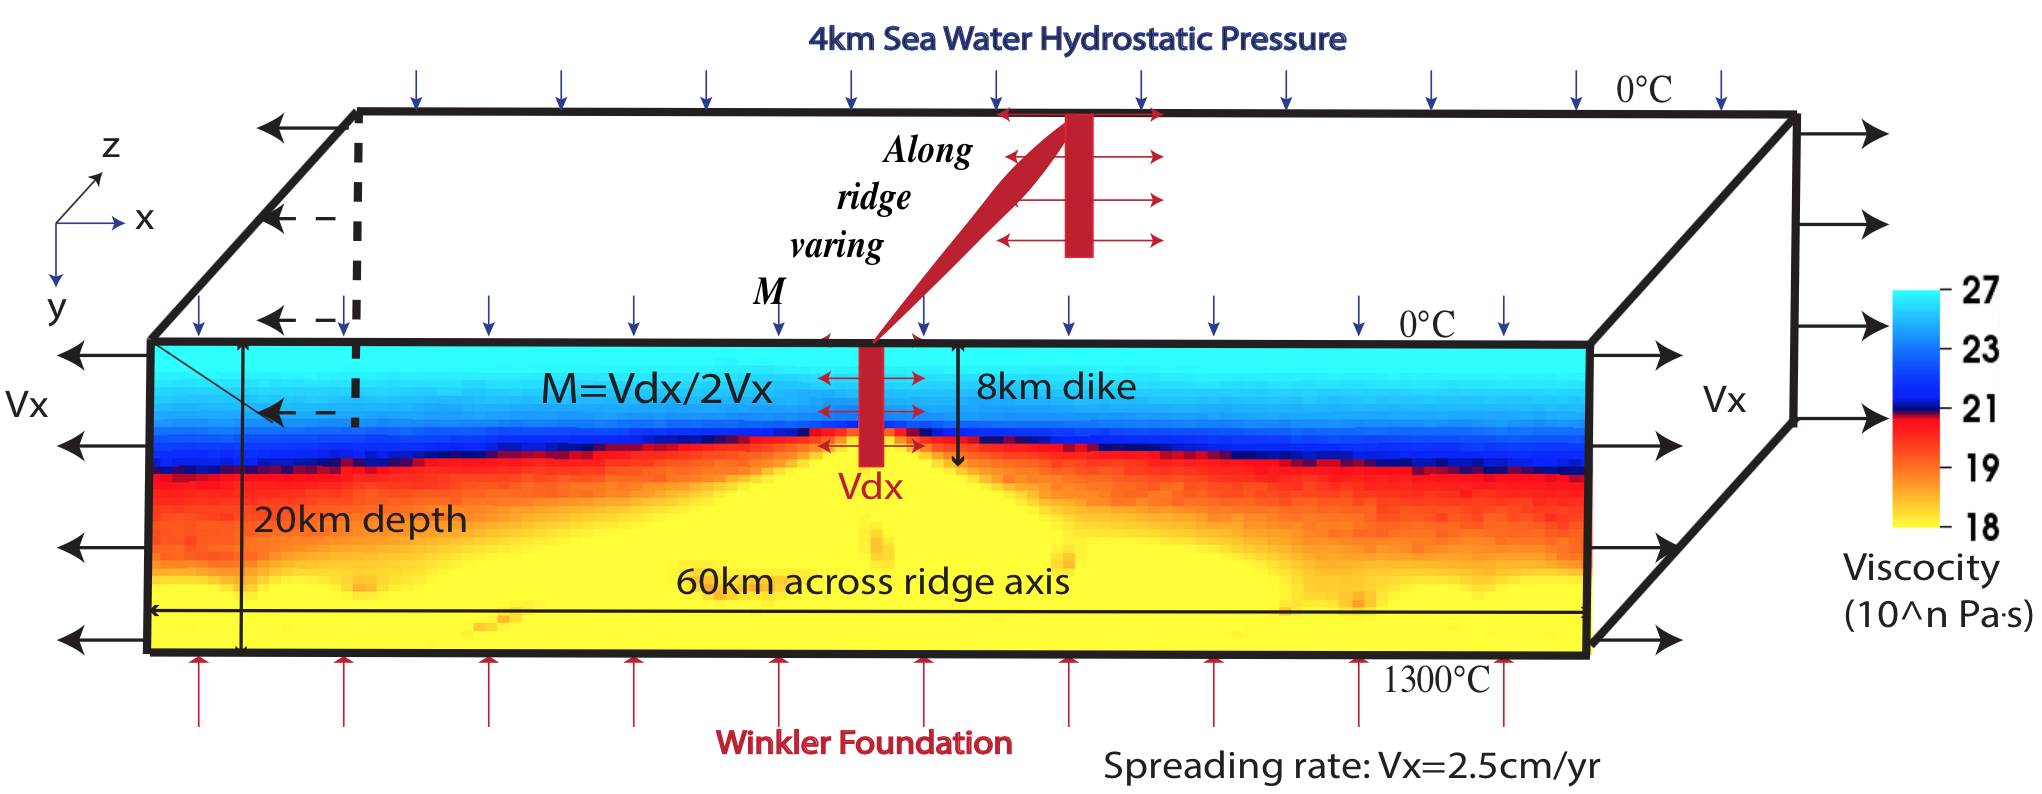
\includegraphics[scale=0.5]{fig8_1.png}
 \caption{\small Preliminary model setup}
 \label{fig8_1}
\end{figure}

Although how to estimate the M values from observations has not been well established, we do have constraints from a large dataset of bathymetry, gravity and seismic surveys as well as geological drilling. Generally, at slow spreading ridges, magma supplies mostly at the center of the ridge segment and decreases towards the end of the segment \citep{Tolstoy1993,Chen1999}. There is also evidence for shorter wavelength of 10 to 20 km discrete focus of magma accretion along the ridge axis \citep{Lin1990}. Based on these constraints, we can start considering only a few end-member scenarios of variations in M along the ridge axis. 

We will experiment on different patterns of M variation. The variation in M is parametrized in terms of the functional forms (e.g. discrete increment, linear, sinusuidal and square root), its wavelength (e.g. 10km, 20km and 40km) and the ranges of M (e.g. 0.2 to 0.8, 0.5 to 0.7 and 0.5 to 0.8). Preliminary pseudo-2D results show that the model behavior in faulting pattern is sensitive to the rate of strain weakening. Two cases of strain weakening will be tested in my thesis. In one case (denoted as Type 1), cohesion linearly decreases from 44 MPa to 4 MPa for plastic strain accumulating from 0 to 0.1. The other case (Type 2) assumes cohesion linearly decreasing from 44 MPa to 4 MPa for plastic strain accumulating from 0 to 0.33.

%\note[EC]{Describe what parameters and what range of their values you are going to explore and why.} \note[XT]{this part is crucial for the project and will be finished after two work being done: 1) thoroughly parameters survey on models we have, based on that understanding will help we proposed what model parameters to be texted; 2) thorough literature review on how M should varies along ridge axis and maybe statistically study on topography along ridge axis from GeoMapApp. }



\break
\section{Work Plan}
\label{ch:plan}

Table \ref{tab:plan} shows what have been done so far and what still need to be finished for the completion of the research.

\begin{table}[hc]
\begin{small}
\begin{center}
\begin{tabular}{|l|p{7cm}|l|}
\hline
Timeline & Work & Progress\\
\hline
Dec., 2013$\sim$Jan., 2014& Understand the basics of MORs tectonics and magmatism system & completed\\ \hline
Jan., 2014$\sim$March, 2014& run 2D models in FLAC to understand the framework& completed\\ \hline
March, 2014$\sim$May, 2014& Learn C programing and continuum mechanics and understand the 3D code& completed\\ \hline
May, 2014$\sim$July, 2014& Benchmark pseudo 3D code with previous modeling results& completed\\ \hline
July, 2014$\sim$Sept., 2014& Implement varying M into 3D code SNAC& completed\\ \hline
Sept., 2014$\sim$Nov., 2014& Run preliminary 3D models and explain the model behaviors& completed\\ \hline
Nov., 2014$\sim$Dec., 2014& Prepare AGU conference poster and presentation& completed\\ \hline

Jan., 2015$\sim$Feb., 2015  & Run different scenarios of M and systematically examine how M affect the topography & ongoing\\ \hline
Feb. 2015$\sim$March, 2015 & Thesis writting & ongoing\\ \hline
April. 2015 & Thesis defense & \\ \hline
\end{tabular}
\end{center}
\end{small}
\caption{An overview of what have been done and plan for what need to be done}
\label{tab:plan}
\end{table}

%\pagebreak
%\section{Budget}
%\label{ch:budget}
%Since observations(topography data of mid-ocean ridges) are handy from GeoMapApp, we don’t need to conduct side scan sonar survey in the deep ocean. GeoMapApp can provide very good bathymetry data and images for this research topic. The software as well as the data are free. We might need some other geophysical evidence (seismology, gravity, resistivity, magnetic etc.) to further support results of the model. They can be attained from other people’s research results. Most of the time will be invested in an iteration process—computer calculations on the 3D model and adjustment on the settings of the model and then calculate again based on previous results. Jobs are run on Super computers Stampede and Penguin. They are our HPC expenses.


\break
\begin{footnotesize}
\bibliographystyle{abbrvnat}
\bibliography{Thesis_Proposal.bib}


\end{footnotesize}

\end{document}